\documentclass[12pt,a4paper]{article}

\usepackage[utf8]{inputenc}
\usepackage[T2A]{fontenc}
\usepackage[ukrainian]{babel}

\usepackage{geometry}
\geometry{left=2cm,right=2cm,top=2cm,bottom=2cm}
\usepackage[table]{xcolor}
\usepackage{graphicx}
\usepackage{placeins}
\usepackage{array,multirow}
\usepackage{booktabs}
\usepackage{caption}
\renewcommand{\thetable}{№\arabic{table}}
\renewcommand{\thefigure}{\arabic{figure}}
\captionsetup[table]{name=Таблиця}

\usepackage{amsmath}
\usepackage{pdflscape}
\usepackage{hyperref}

\usepackage{subcaption}

\usepackage{minted}

\usemintedstyle{vs}
\setminted{linenos, breaklines, frame=single, fontsize=\small}

\begin{document}

    \begin{titlepage}

        % Картинка шапки (по центру, з відступом від верху)
        \begin{center}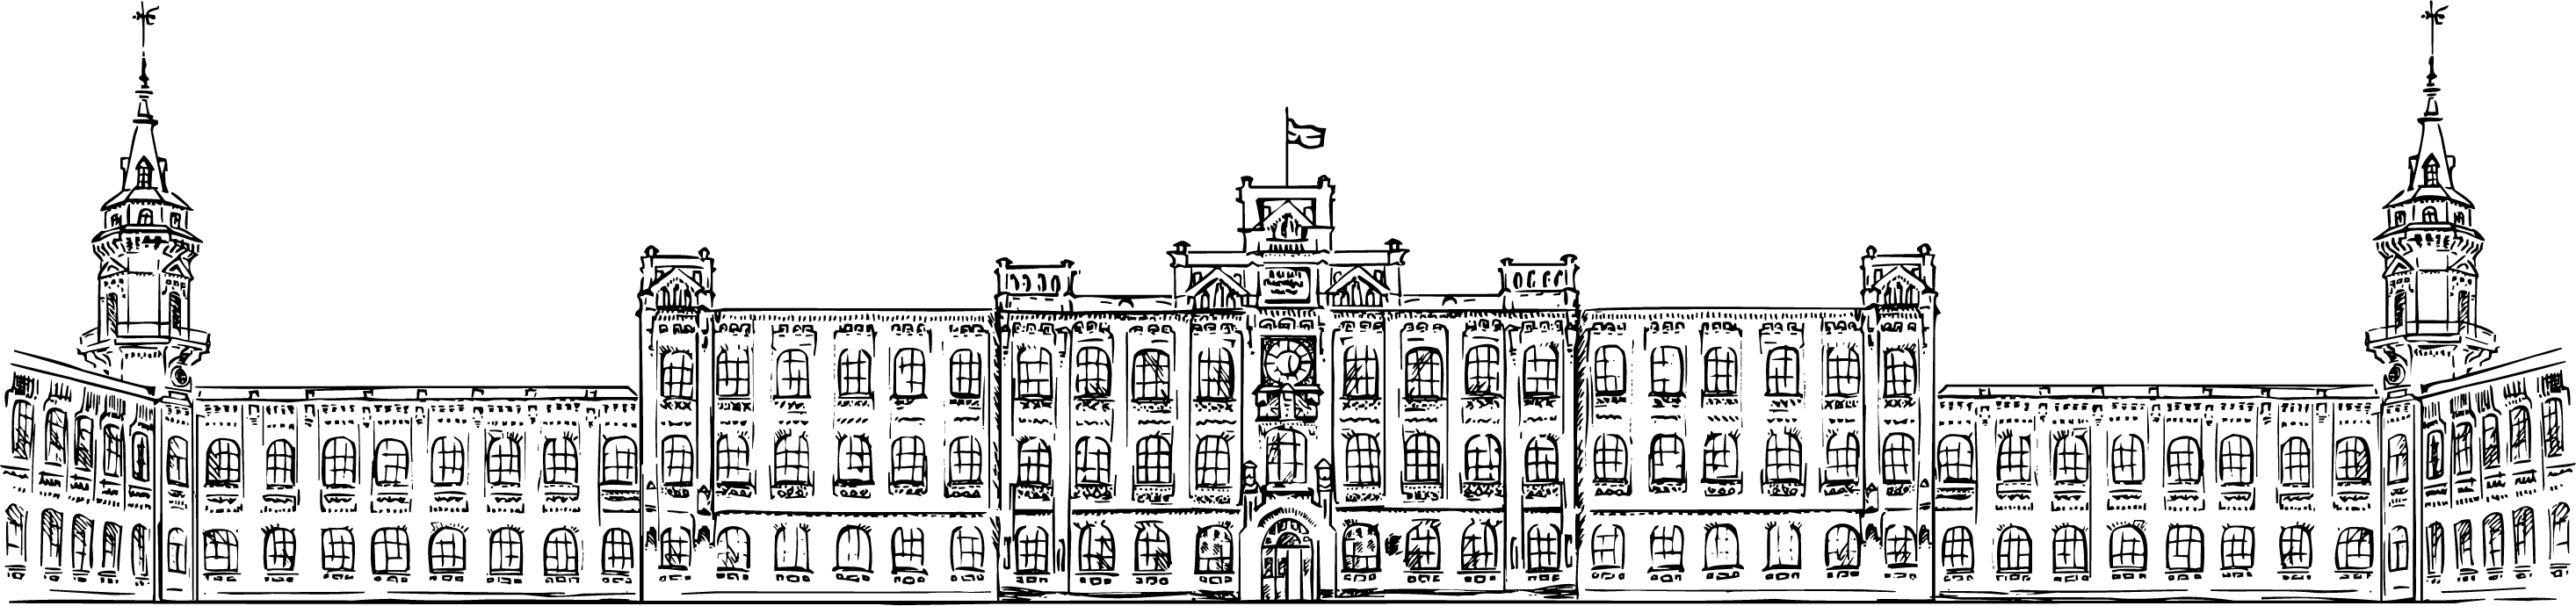
\includegraphics[width=0.7\textwidth]{../../../TITLES/letterhead.png}\end{center}

        \begin{center}
            \large Національний технічний університет України\\
            «Київський політехнічний інститут імені Ігоря Сікорського»\\[1em]
            Факультет інформатики та обчислювальної техніки\\
            Кафедра обчислювальної техніки
        \end{center}

        \vfill

        \begin{center}
            \textbf{\LARGE Практична електроніка}\\[2em]
            \textbf{\Large Лабораторна робота №9}\\[0.5em]
            «Реалізація аналогового компаратора на базі Arduino»
        \end{center}

        \vfill

        \begin{flushright}
            Виконав: студент 2 курсу ФІОТ, гр. ІО-41\\
            \textit{Давидчук А.~М.}\\[1em]
            Перевірив: \textit{Гайдай А.~Р.}
        \end{flushright}

        \vfill

        \begin{center}Київ --- 2025\end{center}

    \end{titlepage}

    % Основний документ:

    \setlength{\parindent}{1.5em}

    \noindent
    \textbf{\underline{Тема:}} «Реалізація аналогового компаратора на базі Arduino».
    
    \vspace{1em}

    \noindent
    \textbf{\underline{Мета:}} реалізувати роботу аналогового компаратора на базі Arduino та дослідити його реакцію на зміну вхідної напруги.

    \begin{center} \textbf{\Large Практична частина} \end{center}

    Мій порядковий номер у списку групи: 6, звідси маю таку плату та таку кількість світлодіодів:

    \begin{itemize}
        \item Плата: esp32-s3;
        \item Світлодіоди: 2 шт.
    \end{itemize}

    \noindent
    Звідси побудую таку схему:

    \begin{figure}[h!]
        \centering
        
\includegraphics[width=0.8\textwidth]{scheme.png}
        \caption{\centering Схема із використанням вбудованого компаратора напруги для керування світлодіодами.}
    \end{figure}

    \noindent
    Що містить:

    \begin{itemize}
        \item Плату esp32-s3;
        \item Потенціометр (значення змінюється повзунком);
        \item 2 світлодіоди з відповідними резисторами обмеження струму (220 Ом).
    \end{itemize}

    \newpage

    \noindent
    \textbf{\underline{Arduino код для плати esp32-s3 (\texttt{sketch.ino}):}}

    \begin{minted}{cpp}
// Реалізація аналогового компаратора на базі ESP32-S3

const int ANALOG_PIN = 1;  // GPIO1 - вхід від потенціометра
const int LED_RED   = 36;  // GPIO36 - Червоний LED, коли напруга НИЖЧЕ порогу
const int LED_WHITE  = 0;  // GPIO0 - Білий LED, коли напруга ВИЩЕ порогу

const int threshold  = 2048;  // порогове значення, що еквівалентне 1.65 В

void setup() {
  pinMode(LED_RED, OUTPUT);
  pinMode(LED_WHITE, OUTPUT);

  digitalWrite(LED_RED, LOW);
  digitalWrite(LED_WHITE, LOW);
}

void loop() {
  int value = analogRead(ANALOG_PIN);  // зчитуємо аналоговий сигнал (0..4095)

  // Компаратор: порівнюємо із threshold
  if (value > threshold) { // вхідна напруга вище за порогову
    digitalWrite(LED_WHITE, HIGH);
    digitalWrite(LED_RED, LOW);
  } else { // вхідна напруга нижче або дорівнює пороговій напрузі
    digitalWrite(LED_WHITE, LOW);
    digitalWrite(LED_RED, HIGH);
  }

  delay(100);  // 100 мс між вимірюваннями
}
    \end{minted}

    \noindent
    Весь проект можна знайти за посиланням: \href{https://wokwi.com/projects/449965876040271873}{Проект на Wokwi}.

    \newpage

    \noindent
    Демонстрація роботи схеми у 2 станах:

    \begin{figure}[h]
        \centering
        
        \begin{subfigure}[t]{0.48\textwidth}
            \centering
            
\includegraphics[width=\linewidth]{test1.png} % перше фото
            \caption{\centering Напруга нижче порогової -- 1 світлодіод (червоний) світиться}
        \end{subfigure}
        \hfill
        \begin{subfigure}[t]{0.48\textwidth}
            \centering
            
\includegraphics[width=\linewidth]{test2.png} % друге фото
            \caption{\centering Напруга вище порогової -- 2 світлодіод (білий) світиться}
        \end{subfigure}
        \caption{Демонстрація роботи схеми}

    \end{figure}

    \noindent\textbf{\underline{Висновок:}} У ході роботи було реалізовано аналоговий компаратор на базі плати ESP32-S3 із використанням вбудованого АЦП. Для порівняння аналогового сигналу від потенціометра було обрано порогове значення 2048 одиниць АЦП. Оскільки ESP32-S3 має 12-бітний перетворювач (діапазон 0..4095), порогова напруга визначалась за формулою
\[
U_{\text{пор}} = \frac{2048}{4095} \cdot 3{,}3 \approx 1{,}65~\text{В},
\]

що становить приблизно половину робочого діапазону. При напрузі на вході SIG нижче 1,65~В спрацьовував червоний світлодіод, а при більшій напрузі — білий, що відповідає принципу роботи компаратора напруги. Схема працювала коректно, а поставлену мету роботи виконано.

\end{document}